\documentclass{abnt}
\usepackage[utf8]{inputenc}
\usepackage[english,brazilian]{babel}
\usepackage{hyperref}
\usepackage{url}
\usepackage{indentfirst}
\usepackage{blindtext}
\hypersetup{%
    pdfborder = {0 0 0}
}
\usepackage{graphicx}
\graphicspath{{./imagens/}}
\usepackage{placeins}

\begin{document}

\autor{Rafael Tavares Amorim \\ Juliano R. Macedo\\ Wolmir L. F. Nemitz}

\titulo{Entrega 2: Gestão de Disponibilidade \\ Versão 1.0}

\instituicao{Universidade Federal do Pampa \par Engenharia da Software \par Resolução de Problemas V}

\local{Alegrete - RS, Brasil}

\data{19 de Maio de 2012}

\capa

\folhaderosto

\tableofcontents


\chapter{INTRODUÇÃO}

	Este relatório tem por finalidade apresentar a fundamentação teórica e tecnológica utilizada no segundo sprint, bem como o detalhamento de nossa solução, e por fim um link de referência para acesso ao sistema.


	
	\section{Metodologia Ágil}
	
		Metodologia ágil é um famoso conjunto de metodologias de desenvolvimento de software, 
		com foco na mitigação dos riscos esta metodologia aposta em pequenos ciclos iterativos de desenvolvimento do software,
		onde ocorre a repetição de cada tarefa comum em um processo de software, ou seja, em cada ciclo realiza-se analise, projeto,
		implementação e testes, referentes aquele módulo, desta forma busca-se à capacidade real de implantar-se um nova versão 
		do software ao final de cada iteração. Ao final de cada clico de iteração a equipe responsável por todo o projeto é reunida 
		e reavalia-se as características, metas e prioridades do projeto como um todo, para que estas sejam aplicadas no próximo ciclo.
		
		Os modelos ágeis são hoje a principal alternativa as metodologias tradicionais de desenvolvimento de software, 
		as quais apresentam diversos problemas estruturais que comprometem a maioria dos projetos, 
		baseados nas necessidades atuais do mercado de software.
	
	\section{Scrum}
	
		\subsection{Visão Geral}
		
			O \emph{scrum} é uma metodologia ágil, muitos consideram como um framework ágil também, que vem cada dia sendo mais popular
			no desenvolvimento de software. O \emph{scrum} tem o objetivo de agilizar o processo de desenvolvimento de software com entregas aos 
			clientes de forma iterativa e com incrementos de software com alto valor. Basicamente temos 3
			papéis neste processo: \emph{Team, Scrum Master e Product Owner}.
		
		\subsection{Papéis}
		
			O \emph{product owner} é um papel muito importante no \emph{scrum}, cabe a ele definir quais funcionalidades devem ou
			não existir no sistema por meio de \emph{user stories} e também definir a prioridade delas. Este papel também
			trata de aprovar ou rejeitar o trabalho realizado e dizer se foi realizado como esperado.
			
			O \emph{scrum master} tem papel de manter a produtividade da equipe, facilitando o processo de \emph{scrum} e resolver impedimentos
			no decorrer do \emph{sprint}. Ele ajuda o time a se manter organizado e certificar que as regras do processo estão sendo
			seguidas corretamente. O \emph{scrum master} não dita o que o time deve fazer mas sim ajuda o time se manter autônomo,
			organizado e com uma boa produtividade. 
			
			O \emph{team} tem papel de transformar os itens de \emph{backlog} em produtos que serão entregues de forma incremental em cada
			sprint. Cabe ao time ter autonomia própria para se organizar e trabalhar de forma de colaborativa ajudando uns aos
			outros sem a necessidade de existência de um "chefe" para dizer o que deve ser feito.
		
		\subsection{Processo}
		
			O processo de \emph{scrum} é trabalhado em cima de vários ciclos chamados de \emph{sprint}, que possuem um tempo fixo, geralmente de
			1 a 4 semanas. Para cada \emph{sprint} é realizado a escolha de \emph{user stories} que estão no \emph{product backlog}. No \emph{product backlog} temos uma lista priorizada 
			pelo \emph{product owner} das funcionalidades desejadas do projeto, e parte desta lista irá forma o \emph{sprint backlog}. É uma coleção de \emph{user stories}.
			
			Em um ciclo, o time irá realizar o \emph{sprint backlog} que contêm os itens de \emph{backlog} que o time concordou 
			completar em um ciclo de \emph{sprint}, cada item de \emph{backlog} é quebrado em tarefas, atribuídas para equipe e estimado o tempo de realização.
			
					
			O \emph{backlog item} ou também conhecido como \emph{user story} é um recurso/funcionalidade desejada no sistema que vão compor o
			\emph{product backlog}. Uma \emph{user story} usualmente é composta por um ator do sistema e a ação para alcançar determinado
			objetivo. Exemplos: 
				\begin{itemize}
					\item Como um <usuário> Eu posso <realizar ação> para alcançar <determinado objetivo>
					\item Como um cliente, eu posso criar um perfil no sistema
					\item Como um cliente, eu posso escolher um usuário e senha
					\item Como um administrador, eu posso bloquear contas de clientes
				\end{itemize}
					 
					
			No \emph{sprint planning}, a equipe decidirá quais \emph{backlog itens} irão para o \emph{sprint backlog}. Depois da priorização das \emph{user
			stories} pelo \emph{product owner}, a equipe seleciona o item do topo do \emph{product backlog}, o qual tem maior prioridade, para a
			discussão e criação das tarefas necessárias para entrega do item. Então as tarefas são atribuídas e estimadas em
			tempo, este processo é repetido até que o time decida que não há possibilidade de realização de mais itens.
			
			Com a ajuda do\emph{Burndown} que é um gráfico que oferece uma forma poderosa que podemos analisar o andamento do projeto. Podemos estimar a velocidade de andamento do time, atrasos e tempo de 
			execução de cada \emph{user story}.
			
			Por meio de um reunião diariamente, podemos também verificar impedimentos que podem afetar a produtividade da equipe, conhecida como \emph{daily meeting}, 
			é uma reunião com duração aproximada de 15 minutos,	conduzida pelo \emph{scrum master} e tem como foco 3 perguntas para todo membro da equipe:
				\begin{itemize}
					\item O que eu fiz ontem?
					\item O que eu estou fazendo hoje?
					\item O que está me impedindo de fazer?
				\end{itemize}
			
			Apesar da reunião ser conduzida pelo scrum master, cada membro deve responder para o time inteiro e não somente para o
			\emph{scrum master}, todos devem estar de pé na reunião e falar somente quando for perguntado pelo \emph{scrum master}. No final da
			reunião é discutido por todos soluções caso haja algum impedimento.
			
			No final de um \emph{sprint}, ocorre uma reunião informal, chamada \emph{sprint review} que tem intuito de demonstrar o que foi 
			realizado no sprint com a presença da equipe, \emph{scrum master}, \emph{product owner} e stakeholders. Também é feita a reunião chamada \emph{sprint retrospective}
			que é uma reunião da equipe que tem objetivo de discutir se o \emph{sprint} foi realizado com sucesso ou se é necessário melhorias.
			
			Um projeto em \emph{scrum} pode ser parado a qualquer momento, as vezes o cliente percebe que as funcionalidade implementadas já foram
			suficientes e atendem a necessidade atual assim não dispersando dinheiro em funcionalidade que talvez nunca seriam utilizadas.
			
			As informações desta seção foram retiradas da referência \cite{SCRUMEPF}.
	
	\section{Python}
	
		\emph{Python} é uma conceituada linguagem de programação de alto nível, interpretada, orientada a objetos e de tipagem forte. Idealizada como uma linguagem que valorize o tempo e esforço do programador, Python foca a legibilidade do código, sua indentação, velocidade de desenvolvimento e expressividade. Dentro desta filosofia 
		podemos destacar a forte indentação da linguagem, o que facilita a sua leitura melhorando o visual organizacional da linguagem, e também sua sintaxe simples, limpa e coerente coopera para um rápido aprendizado.\cite{PYTHON}
	
	\section{Pip}
	
		Devido à grande quantidade de extensões, bibliotecas e frameworks que utilizam o \emph{Python}, a comunidade dessa linguagem criou um repositório centralizado de pacotes, o \emph{Python Package Index}.
		\emph{Pip} é uma ferramenta para instalar e gerenciar pacotes \emph{Python}, tais como aqueles encontrados no \emph{Python Package Index}.\cite{PIPSITE}

	\section{Django}
		\emph{Django} é um framework para desenvolvimento web em Python, cuja proposta
		é encorajar a construção rápida e pragmática de aplicações.\cite{DJANGOSITE}
		O \emph{django} segue a arquitetura model-view-controller. O modelo das aplicações
		é definido através de classes de modelo que serão mapeadas, mediante o lançamento do projeto,
		para entidades relacionais no banco de dados definido pelos desenvolvedores. A \emph{view} é
		representada através de funções ou métodos que processam requisições com um sistema
		de templates. O \emph{controller} é nada mais que a customização das URLs da aplicação,
		que podem ser detectadas através de expressões regulares e redirecionam o
		usuário à \emph{view} apropriada.\cite{DJANGOWIKIPEDIA}
	
	\section{South}
		\emph{South} é uma ferramenta de migração de dados em aplicações \emph{Django}, 
		permite ao desenvolvedor migrar as informações do banco de dados apos refatorações no modelo
		sem que seja necessário manipular-se o banco, executando as alterações necessárias 
		no mesmo de acordo com as modificações realizadas.
				
		Suas principais característica são: 
			\begin{itemize}
			\item Criação e migração automática: South pode ver o que realmente foi modificado no seu arquivo models.py
			 e automaticamente escrever a migrações que corresponda as suas alterações.
			\item Independência de banco de dados: Na medida do possível, do \emph{South} é completamente independente 
			de banco de dados, suportando atualmente cinco \emph{backends} de bancos de dados diferentes.
			\item Avançado: \emph{South} reconhece e trabalha com o conceito de aplicativos \emph{Django}, permitindo que você use 
			as migrações para as aplicações que você preferir, e deixa-lhe trabalhar sobre syncdb nas demais.
			\end{itemize}
			
		As informações desta seção foram retiradas da referência \cite{SOUTH}.
	
	\section{Jenkins}
			
				\emph{Jenkins} é um servidor de integração contínua de código fonte aberto escrito em Java, e com mais de 300 plugins para
				suportar diferentes tipos de desenvolvimento de software. O \emph{Jenkins} prover o processo de integração contínua para o
				desenvolvimento de software \cite{JENKINS}.
				
				O processo de integração contínua visa melhorar a qualidade de software e reduzir o tempo de entrega, substituindo a
				prática tradicional de aplicação do controle de qualidade depois do desenvolvimento completo. Os princípios da
				integração contínua são\cite{CIWIKIPEDIA}:
				\begin{itemize}
				  \item Manter o código fonte em um repositório de controle de versão
				  \item Automatizar a construção de software
				  \item Fazer a construção de software testar automaticamente o software
				  \item Todo mundo deve comitar para o repositório base todo dia
				  \item Todo commit para repositório base deve ser construído
				  \item A construção deve ser rápida para identificação dos problemas rapidamente
				  \item Testar em um ambiente clone de produção
				  \item Deixar última construção sucedida disponível para os stakeholders e testadores
				  \item Todo mundo pode ver o resultado das últimas construções
				  \item Automatizar o deploy
				\end{itemize}
				
				Sendo importante, a parte de testes para que a integração contínua funcione. Existem mecanismos implementados em
				varias linguagens que podem não somente testar o funcionamento total da aplicação mas como verificar a qualidade de
				código fonte escrito baseado em vários fatores como padrão de codificação, detecção de cópias, detecção de erros em
				syntax e problemas de lógica, também chamado de inspeção contínua.\cite{INSPECAO-CONTINUA}
				
				A ferramenta \emph{Jenkins} entra para a execução do processo de integração contínua, irá tratar de obter o código fonte,
				realizar a construção com ajuda do \emph{Maven}\cite{MAVENBUILDTOOL} ou \emph{Ant}\cite{ANTBUILDTOOL}, realizar a execução dos testes e fazer o deploy para o servidor de
				teste.\cite{JENKINS-BUILD}

		\section{Klaros Testmanagement}
		
			É uma aplicação web baseada em AJAX escrita em Java para organização e gerenciamento do processo de teste. O sistema
			permite a construção dos casos de teste, gerenciar casos de teste, dividir em suítes de testes, cadastrar os
			ambientes de teste e sistemas que estão rodando o teste, executar testes e coletar os resultados.
			
			Pelos testes realizados no sistema, temos a possibilidade da construção de casos de teste, os casos de teste são
			nomeados, descritos (descrição, pré-condição e pós-condição), priorizados entre os demais, possui estado de
			execução, modo de execução e podem ser divididos em vários passos. Também se pode definir o ambiente de execução
			como Sistema Operacional ou Navegador para aplicações Web. A interface do sistema é bem amigável, não houve
			dificuldades de navegação sobre a aplicação.
			
			\begin{itemize}
			  \item Possui versionamento e histórico sobre os dados.
			  \item Trabalha com casos de teste e seus resultados.
			  \item Gera relatórios em gráficos e tabela sobre os testes. Podendo ser exportado em vários formatos como PDF,
			  HTML, entre outros.
			  \item Possui suporte de integração com as ferramentas de gerenciamento de projeto Redmine, Jira, Trac e Bugzilla.
			  \item É possível através de plugin dos sistemas de integração continua (Hudson/Jenkins) importar os relatórios de
			  execução dos testes automatizados.
			  \item Pode ser instalado em Windows por meio de um executável e Linux por meio de um arquivo jar.
			\end{itemize}
			
			A ferramenta se mostrou muito fácil de instalar como um software que você instala no dia a dia com poucos cliques,
			possui um instalador que facilita muito e instalar todas as dependências e o servidor em si. Após a instalação, a
			configuração nada mais foi do que informar o usuário e senha para o administrador assim podendo-se inciar as
			atividades de teste na ferramenta. Para integração com gerenciamento de defeitos, na parte administrativa, é
			informado o gerenciamento de defeito, endereço, usuário e senha. 
			
			Todas informações desta seção foram retiradas da referência \cite{KLAROS}.
			
	\section{MySQL}

		\emph{MySQL} é o sistema de gerenciamento de base de dados mais utilizado no mundo.
		É o \emph{SGBD} utilizado no projeto de gerenciamento de disponibilidades por ser livre de custos
		e amplamente documentado.\cite{MYSQLWIKI}
	
\clearpage

\chapter{SPRINT}
	
		Esta seção aborda as informações sobre o Sprint II, demonstrando o nosso sprint backlog logo a baixo.
	
	\section{Detalhamento da Solução}
	
		Apos a apresentação do problema proposto a equipe trabalhou sobre as propostas de solução que melhor envolviam o ambiente já definido no sprint anterior,
		apos este levantamento determinou-se que o projeto seria construído sobre os seguintes pilares:
		\begin{itemize}
		\item  A linguagem de programação seria Python.
		\item O ambiente de desenvolvimento integrado será à Aptana Studio 3.
		\item O ambiente de desenvolvimento sera Web.
		\item  O framework de desenvolvimento será o Django.
		\item  A ferramenta de gerenciamento será o Redmine.
		\item  A ferramenta de versionamento será o GitHub.
		\item  A ferramenta de gerenciamento e execução de testes será o Klaros.
		\item  A ferramenta de integração contínua será o Jenkins.
		\end{itemize}
		
		Dentro desta primeira versão do sistema, estão inclusos as funcionalidades a seguir:
			\begin{itemize}
			\item Crud de Disciplinas:
			\subitem Cadastro de disciplinas.
			\subitem Visualização dos dados de disciplinas.
			\subitem Edição dos dados de disciplinas.
			\subitem Remoção de disciplinas.
			
			\item Crud de Compromissos:
			\subitem Cadastro de compromisso.
			\subitem Visualização de compromissos.
			\subitem Edição de compromisso.
			\subitem Remoção de compromisso.
			
			\item Crud de Tipo de Salas:
			\subitem Cadastro de tipos de salas.
			\subitem Visualização dos dados de tipos de salas.
			\subitem Edição dos dados de tipos de salas.
			\subitem Remoção de tipos de salas.
			
			\item Crud de Salas:
			\subitem Cadastro de salas.
			\subitem Visualização dos dados de salas.
			\subitem Edição dos dados de salas.
			\subitem Remoção de salas.

			\end{itemize}

	
	\section{User Story 1}
	\subsection{Análise}
		A análise do CRUD de disciplinas foi erroneamente baseada em uma expansão da \emph{user story} abordada na primeira semana. Com isso, a modelagem e, consequentemente, a implementação da funcionalidade não foram totalmente validadas pelos Product Owners.
		Uma nova modelagem já foi discutida pelo grupo e será submetida a validação pelos \emph{product owners} no início do próximo \emph{sprint}.
		
		Realizamos a codificação da user story baseado no levantamento executando junto aos product owners os quais apontaram desejos e necessidades urgentes para tal, todas elas foram atendidas, e esta user story esta cem porcento funcional. 
	
	\section{User Story 2}
	\subsection{Projeto}
	Realizamos a expansão da user story explorando seus casos de uso, e em seguida construímos o diagrama que representava estes casos de uso.
	Apos a implementação de algumas funcionalidades já iniciamos a execução dos testes no sistema, os quais foram gerenciados pela ferramenta já citada, o Klaros, seus relatórios, gerados ao final de cada teste foram salvos e reportados como evidências para o projeto como um todo. 
	
	Na modelagem do cadastro de professores e compromissos, as seguintes relações foram propostas:
	Um professor poderia estar vinculado a várias disciplinas e poderia ter vários compromissos, mas apenas uma área de formação.
	Salas também poderiam ter compromissos.
	A sequencia de mensagens está demonstrado através do diagrama em anexo.
	
	\section{User Story 3}
	
	Durante o projeto da semana três, realizamos a construção do diagrama de classes bem como seu diagrama de sequencia.
	Projetamos a futura arquitetura desta user story a qual pode ser visualizada no diagrama geral, no final desta seção. 
	
	\section{User Story 4}
	
	
		\begin{figure}[h]
			\begin{center}
				 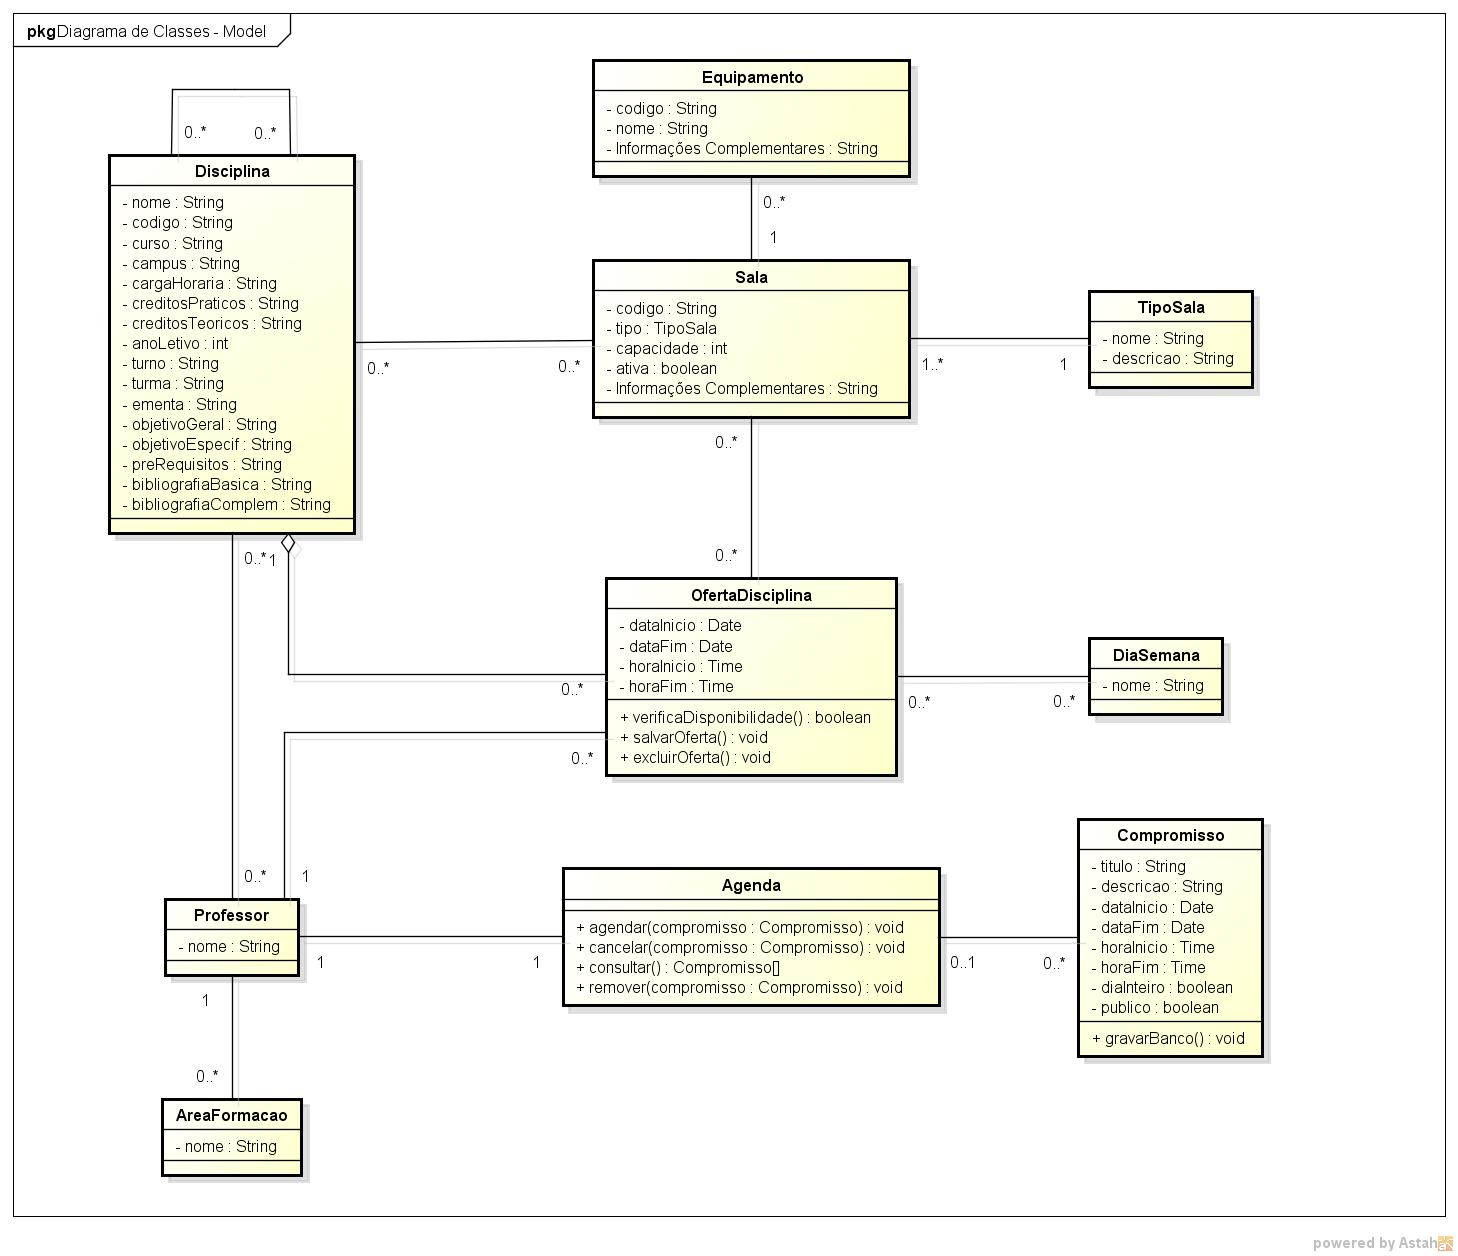
\includegraphics[width=400px]{classesmodelo}
				 \caption[labelInTOC]{Diagrama de Classes Modelo}
				 \label{fig:diagramaClassesModelo}
			\end{center}
		\end{figure}
		\FloatBarrier

	\clearpage

	\section{Acesso ao Sistema}
			De acordo com o planejamento construído no sprint anterior o qual definimos nossa infraestrutura de desenvolvimento, 
			o sistema esta em integração contínua com o servidor de testes on-line, podendo ser acessado a partir da seguinte url:
		
			\url{http://chicago1.vsnetwork.net/}
			

	\section{Acesso as Ferramentas}
		
		O gestor de projeto pode ser acessado através da url: \url{http://redmine.vsnetwork.net/projects/rp-v} , o qual está visivelmente público em todas as atividades do projeto. 
		
		O código fonte do projeto pode ser acessado pelo github\cite{GITHUB} na url: \url{https://github.com/dextervip/rpv}. 
		
		As construções automatizadas do jenkins podem ser acessadas pela url: \url{http://chicago2.vsnetwork.net:8080/job/RPV}.

	\clearpage

	%Referências Bibliograficas
	\nocite{*}
	\bibliographystyle{abnt-num}
	%\bibliographystyle{plain}		
	\bibliography{bibliografia}		

\end{document}